% ============================================================
%  Metódy inžinierskej práce — Cvičenie 4, úloha 7
%  Experimenty s vlastnosťami obrázkov/diagramov (MiKTeX / LaTeX).
%
%  Tento dokument zámerne NEZMENÍ odovzdaný clanok.tex; slúži ako
%  samostatný dôkaz toho, že sme si vyskúšali zmeny veľkosti, rotácie,
%  pozície a zarovnania obrázkov. Rovnaké príkazy sa dajú použiť
%  v ľubovoľnom LaTeXovom projekte (aj v Overleaf).
% ============================================================
\documentclass[10pt,a4paper,slovak]{article}

\usepackage[slovak]{babel}
\usepackage[utf8]{inputenc}
\usepackage[T1]{fontenc}
\usepackage{graphicx}
\usepackage{wrapfig}
\usepackage{caption}
\usepackage{float}
\graphicspath{{../img/}{img/}}  % funguje pri preklade z cv4/ aj z koreňa

\title{Cvičenie 4 — vlastnosti obrázkov a diagramov v \LaTeX{}u}
\author{Matvii Nosenko, Volodymyr Nedoluha, Danylo Nikolenko, Rostyslav Mykytiuk}
\date{\today}

\begin{document}
\maketitle

\noindent
V tomto dokumente systematicky skúšame meniť \textbf{veľkosť}, \textbf{rotáciu},
\textbf{pozíciu}, \textbf{zarovnanie} a \textbf{orezanie} obrázka. Použitý je
diagram \texttt{img/diagram1.pdf} vytvorený v nástroji UMLet/UMLetino.

\section{Veľkosť obrázka}

\noindent Veľkosť sa dá meniť relatívne (\texttt{width}, \texttt{height}),
pomerovo (\texttt{scale}) alebo so zachovaním pomeru strán
(\texttt{keepaspectratio}).

\bigskip
\noindent\textbf{a) predvolená veľkosť (100\,\%):}\par
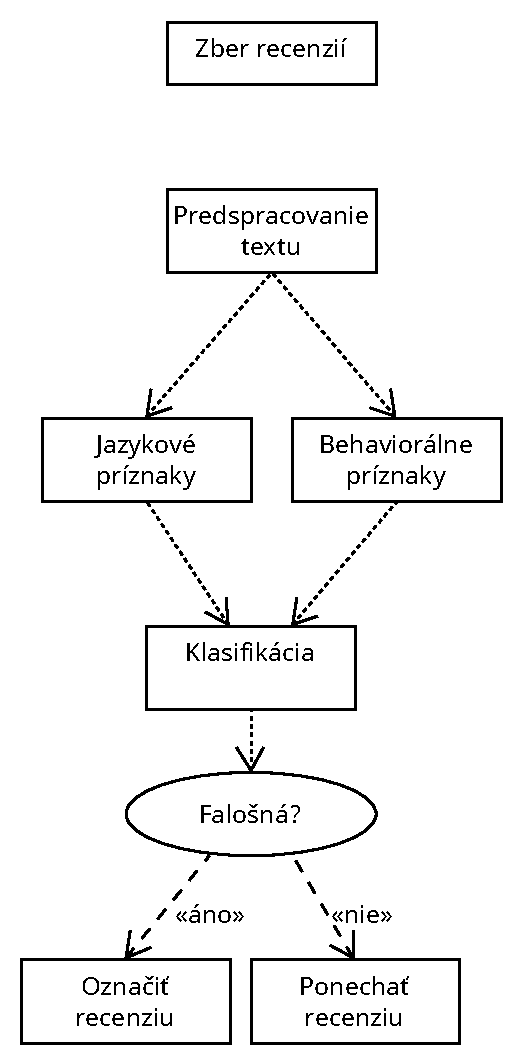
\includegraphics{diagram1.pdf}

\bigskip
\noindent\textbf{b) šírka = 40\,\% šírky riadku:}\par
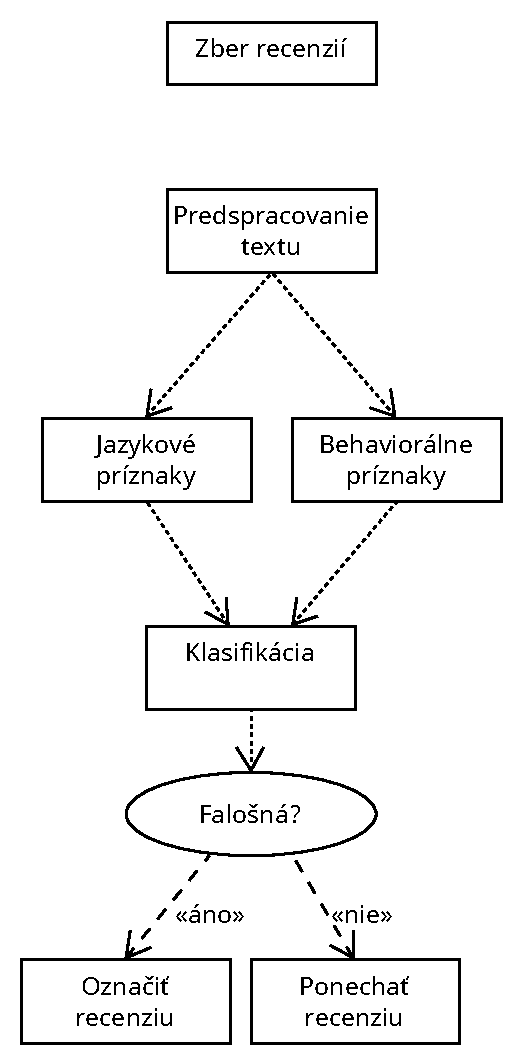
\includegraphics[width=0.4\linewidth]{diagram1.pdf}

\bigskip
\noindent\textbf{c) pomerové zmenšenie \texttt{scale=0.25}:}\par
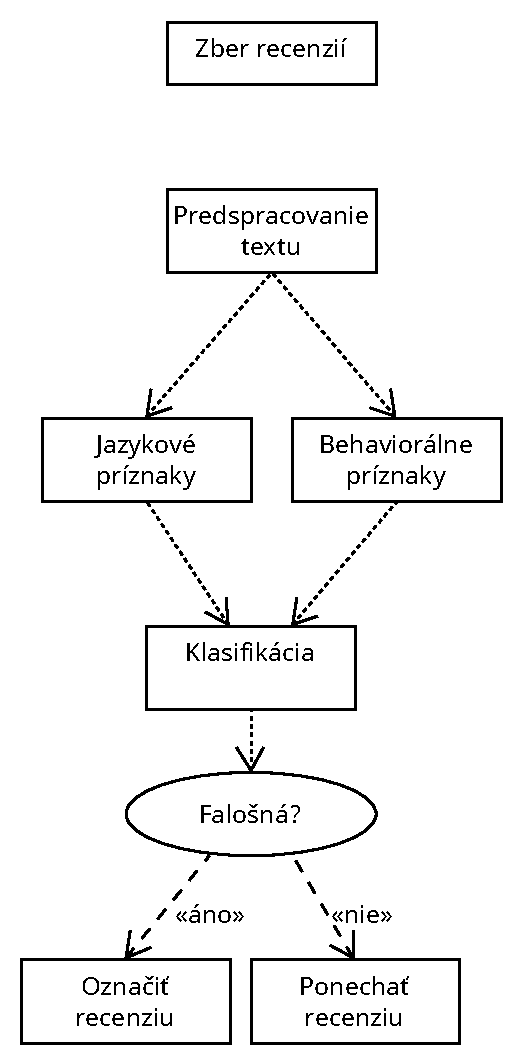
\includegraphics[scale=0.25]{diagram1.pdf}

\bigskip
\noindent\textbf{d) pevná výška so zachovaním pomeru:}\par
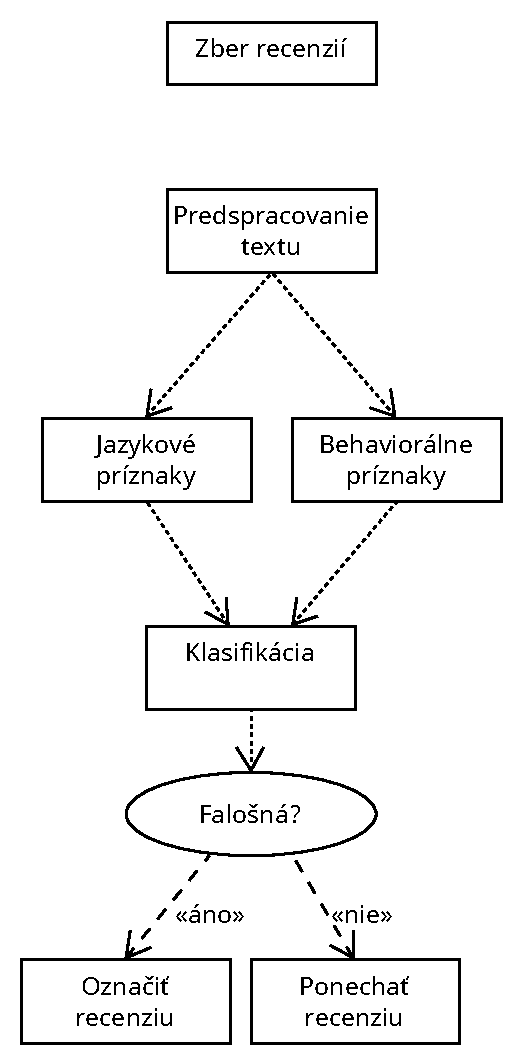
\includegraphics[height=3.5cm,keepaspectratio]{diagram1.pdf}

\section{Rotácia obrázka}

\noindent Otáčanie zabezpečuje parameter \texttt{angle}; parameter
\texttt{origin=c} otáča okolo stredu obrázka.

\bigskip
\noindent
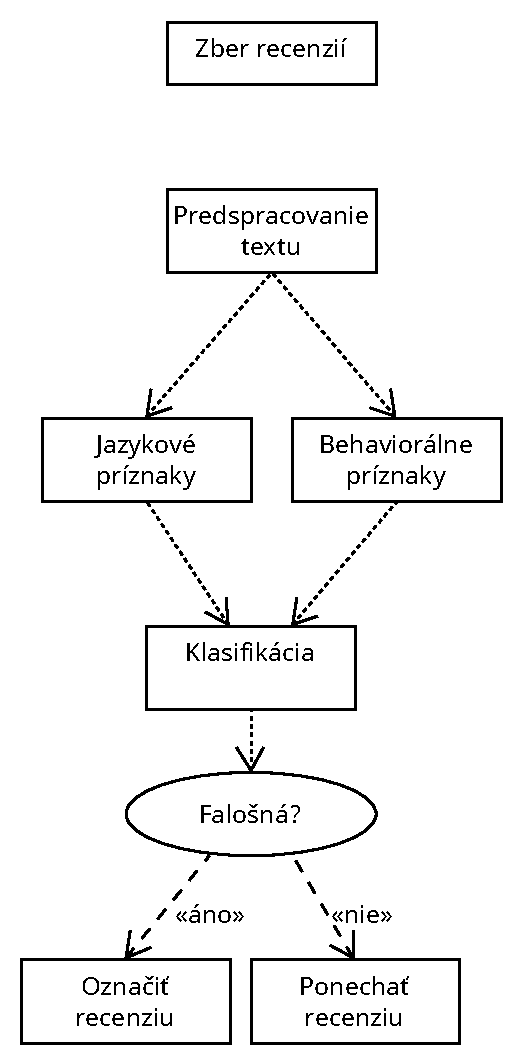
\includegraphics[width=0.25\linewidth,angle=15]{diagram1.pdf}
\hspace{1cm}
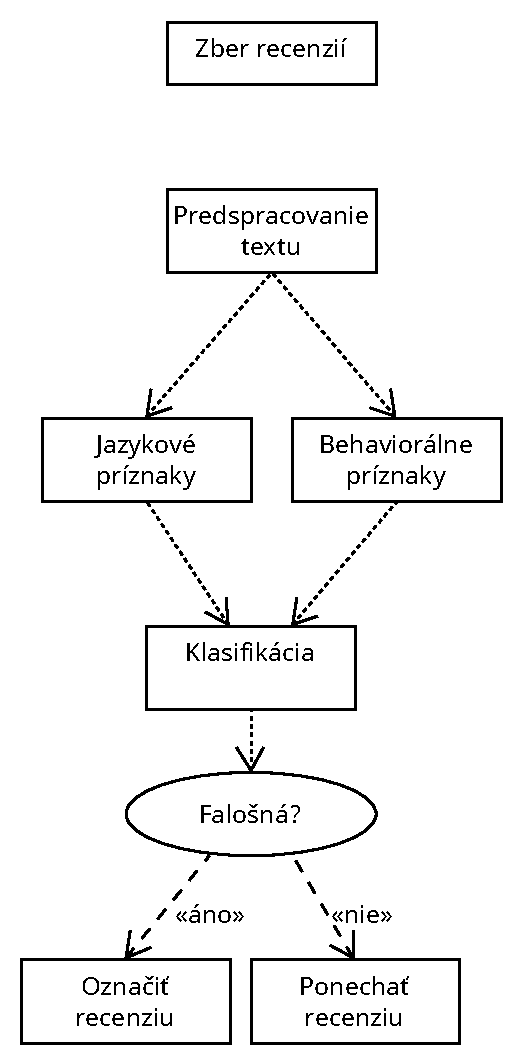
\includegraphics[width=0.25\linewidth,angle=45,origin=c]{diagram1.pdf}
\hspace{1cm}
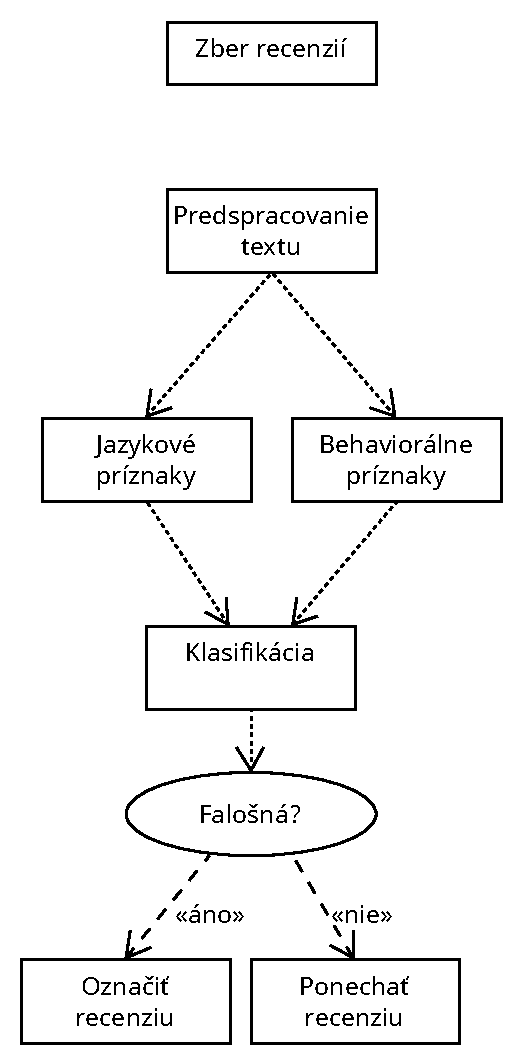
\includegraphics[width=0.25\linewidth,angle=90,origin=c]{diagram1.pdf}

\section{Zarovnanie obrázka}

\noindent Zarovnanie na ľavý okraj, na stred a na pravý okraj:

\bigskip
\noindent\makebox[\textwidth][l]{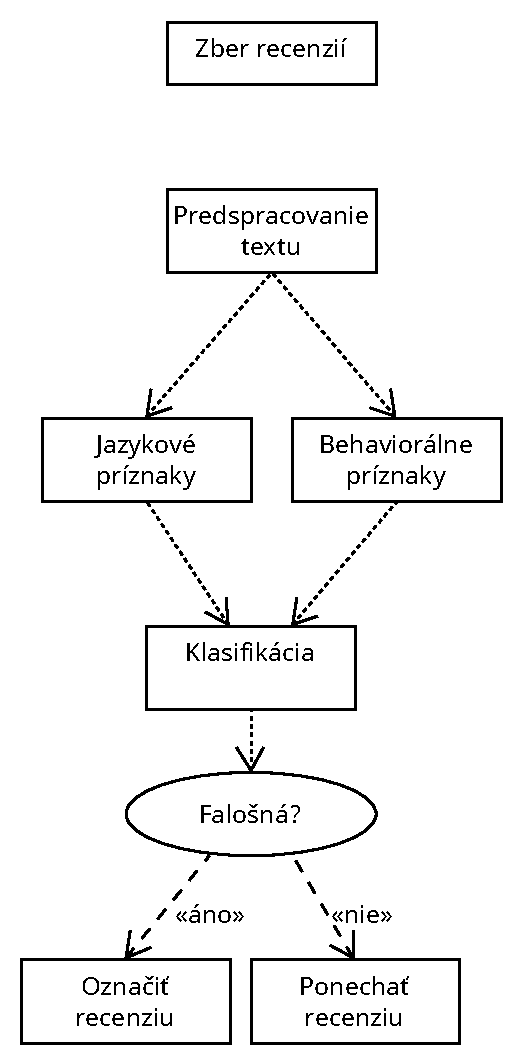
\includegraphics[width=0.2\linewidth]{diagram1.pdf}}\par
\bigskip
\noindent\makebox[\textwidth][c]{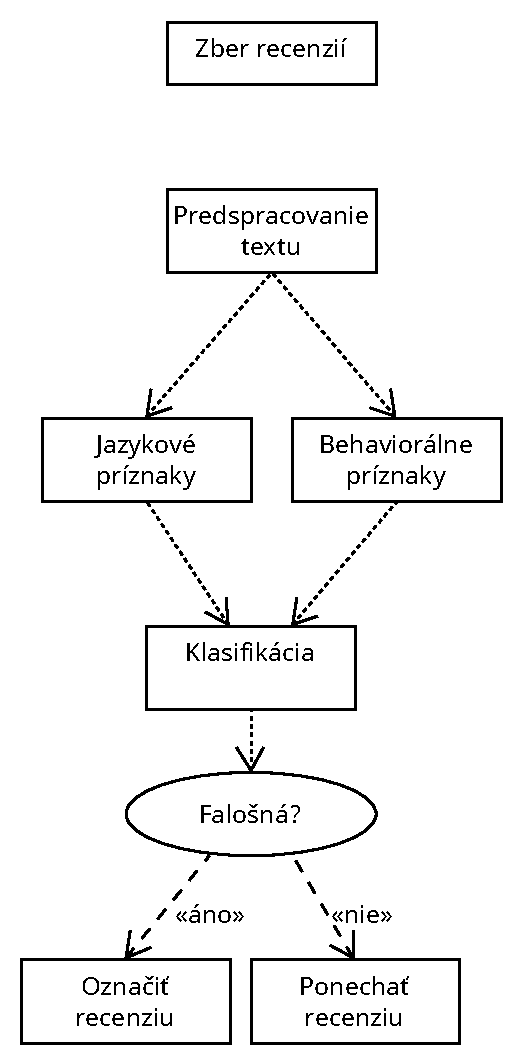
\includegraphics[width=0.2\linewidth]{diagram1.pdf}}\par
\bigskip
\noindent\makebox[\textwidth][r]{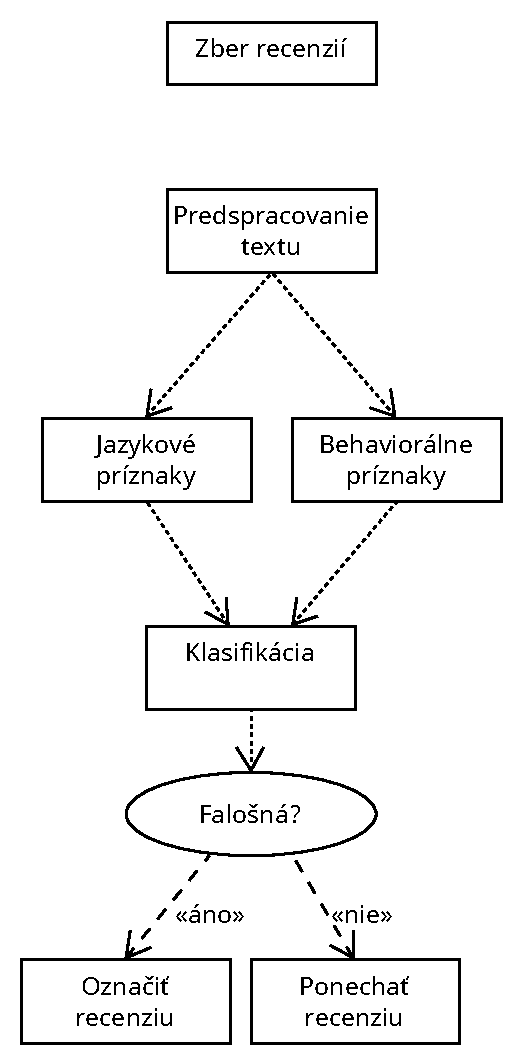
\includegraphics[width=0.2\linewidth]{diagram1.pdf}}\par

\section{Pozícia — plávajúci vs. neplávajúci obrázok}

\noindent V \LaTeX{}u je obrázok v prostredí \texttt{figure} \emph{plávajúci}:
parameter \texttt{[h]/[t]/[b]/[p]} navrhuje, kde ho má sadzač umiestniť.
Neplávajúci obrázok vložíme priamo do textu (napr. v prostredí
\texttt{center} alebo \texttt{minipage}).

\begin{center}
  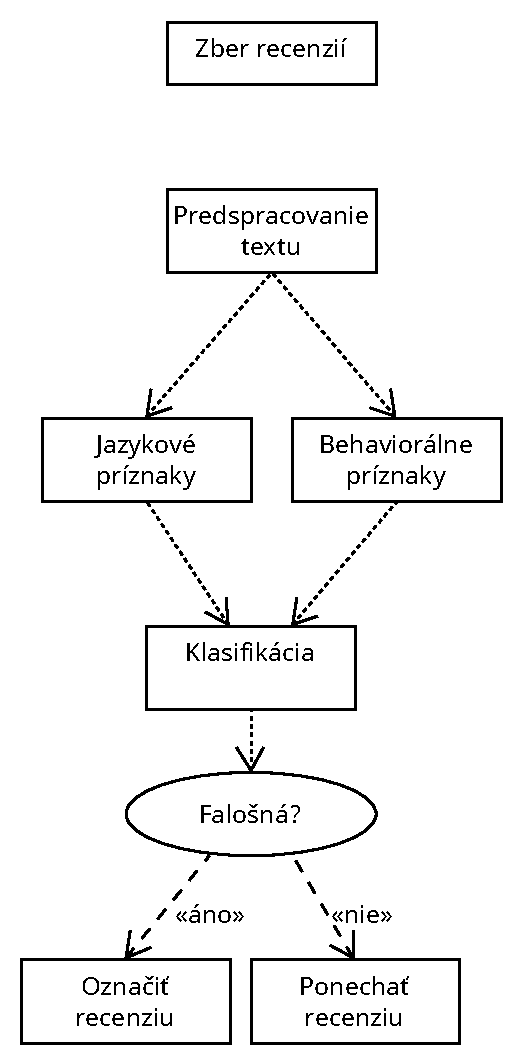
\includegraphics[width=0.35\linewidth]{diagram1.pdf}
  \captionof{figure}{Neplávajúci obrázok vycentrovaný prostredím \texttt{center}.}
\end{center}

\section{Obtekanie textom}

\noindent
\begin{wrapfigure}{r}{0.3\textwidth}
  \centering
  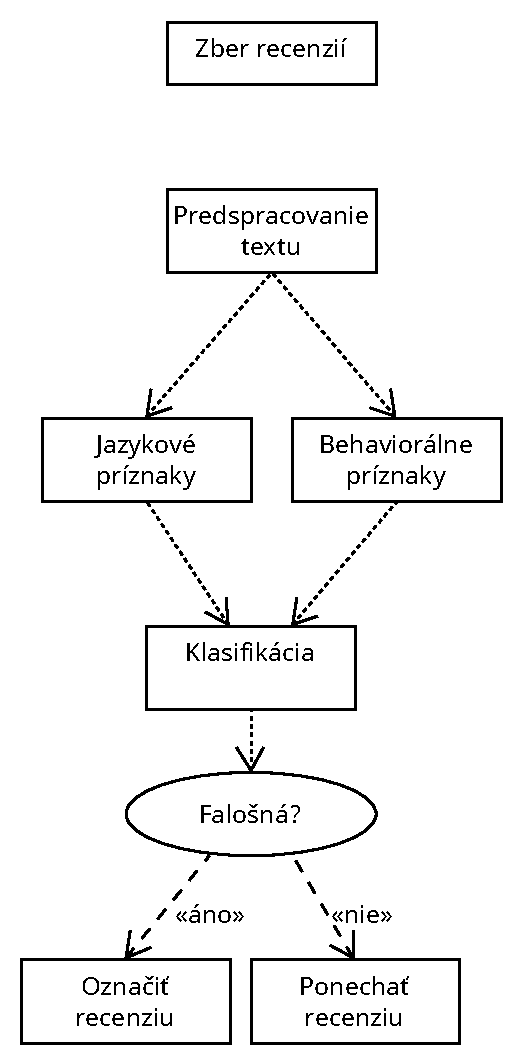
\includegraphics[width=0.28\textwidth]{diagram1.pdf}
  \caption{Obrázok obtekaný textom cez \texttt{wrapfigure}.}
\end{wrapfigure}
Obtekanie textom zabezpečuje balík \texttt{wrapfig}. Obrázok je pripevnený
k pravému okraju a text sa obtáča okolo neho. Takto je vložené aj logo FIIT
v odovzdanom článku (\texttt{clanok.tex}). Text pokračuje dostatočne dlho,
aby bolo obtekanie viditeľné. Text pokračuje dostatočne dlho, aby bolo
obtekanie viditeľné. Text pokračuje dostatočne dlho, aby bolo obtekanie
viditeľné. Text pokračuje dostatočne dlho, aby bolo obtekanie viditeľné.
Text pokračuje dostatočne dlho, aby bolo obtekanie viditeľné. Text pokračuje
dostatočne dlho, aby bolo obtekanie viditeľné. Text pokračuje dostatočne dlho,
aby bolo obtekanie viditeľné.

\section{Orezanie (trim / clip)}

\noindent Orezanie okrajov sa robí parametrom \texttt{trim} v tvare
\texttt{l b r t} spolu s \texttt{clip} (aby zvyšok nepresahoval).

\bigskip
\noindent\textbf{originál:}\quad
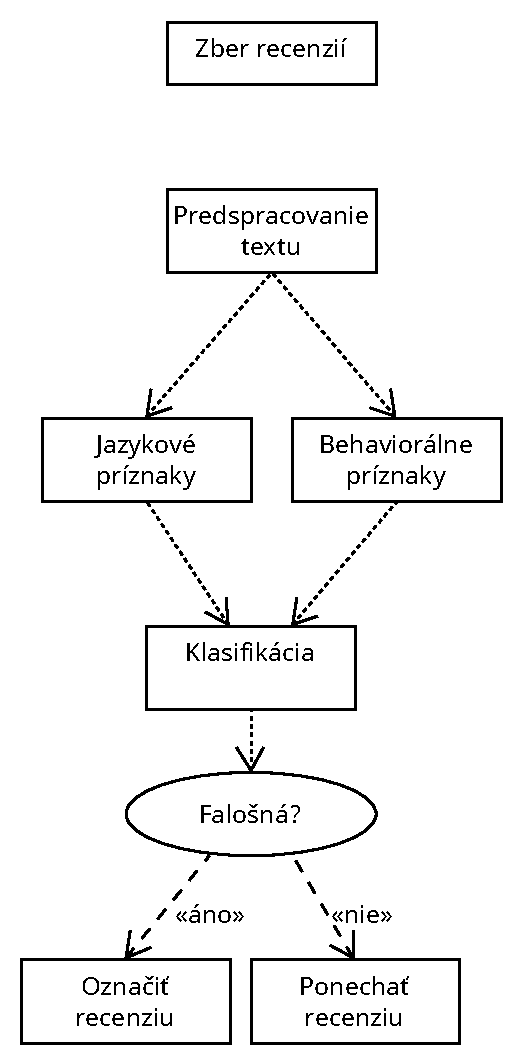
\includegraphics[width=0.25\linewidth]{diagram1.pdf}

\bigskip
\noindent\textbf{orezané \texttt{trim=1cm 1cm 1cm 1cm,clip}:}\quad
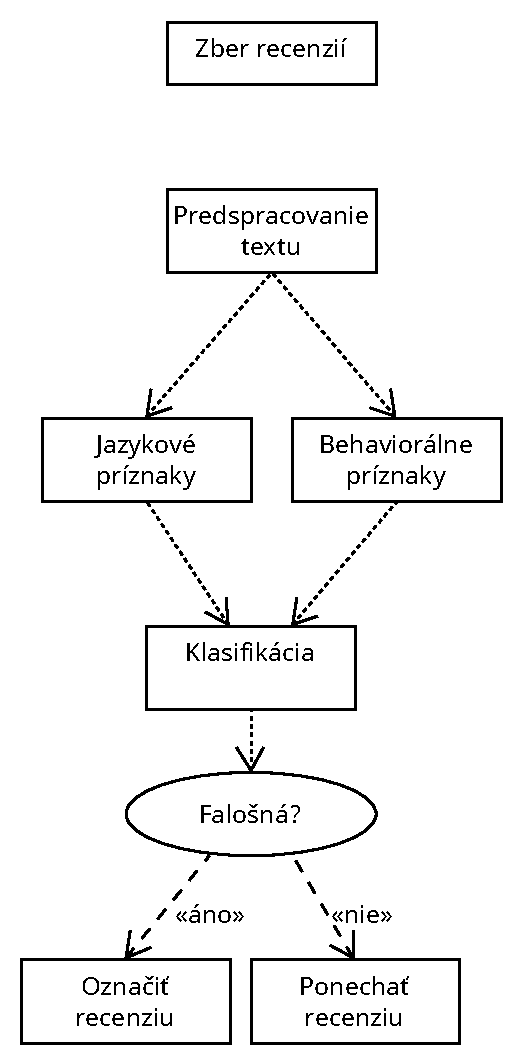
\includegraphics[width=0.25\linewidth,trim=1cm 1cm 1cm 1cm,clip]{diagram1.pdf}

\end{document}
